% =====================================================================================
% FIGURE 1.1 — the experiment on one page.
%
% HOUSE STYLE: docs/figures/specimen_channel.tex, master plan 33.5a. Not re-derived here.
% White fills with thin borders and never a colour block, three colours only, section
% labels over grey rules instead of banner bars, a dimension on every data-flow
% arrow, the feedback loop drawn explicitly and labelled with WHY it exists, and no "..."
% omissions. Colours are Okabe-Ito (Wong, Nature Methods 2011), matching src/viz/style.py.
%
% WHY THIS FIGURE EXISTS. The guide states that the second marker may come from any
% discipline and assesses only the submitted report. This is the one image that hands
% such a reader the entire design: what varies, what is held, and why the comparison
% identifies anything. It replaces roughly 200 words of counted prose with an exhibit
% the word count excludes.
%
% THE LOSSY-STEP CONVENTION IS A SHAPE, NOT A COLOUR. The manipulated block carries the
% vermillion border AND a double rule, because the specimen's greyscale proof found that
% colour alone made the emphasis vanish in black-and-white print.
%
% EVERY NUMBER HERE IS STRUCTURAL OR FROZEN, none is a result: five conditions, six
% statistics, 400,000 steps (amendment R77), and the three split boundaries (Split C).
% Deliberately ABSENT: the per-arm character counts, because CH4's table records
% 270/62/288/81/270 while master plan 28.4 records 67/86/275/293/275 and the two have
% not been reconciled. An unreconciled number does not go into an exhibit.
%
% ------------------------------------------------------------------------------------
% TYPOGRAPHY, RE-FITTED 2026-08-10. Three defects, all measured on the built PDF:
%
%  (1) TYPE SIZE. Every label was set between 6.0 and 7.3 pt against the IFTE0008
%      guideline of Arial/Helvetica at >= 10 pt — the smallest type in the document.
%      The whole layout below is re-fitted at 10 bp (see the note at the tikzpicture
%      options for why bp and not pt): the grid is in cm and the type in points, so
%      raising the size alone would have burst every box. Boxes are therefore
%      sized by \boxwd / \boxwdB and their labels re-wrapped; the arrow dimensions are
%      re-broken to fit the channel that is left. No wording and no number changed.
%
%  (2) COLUMN WIDTH. The drawing measured 425 pt against a 453.5 pt text column, and
%      \pandocbounded never scales UP, so it sat inside the column with white on the
%      right. \W below is the full column less the 4 pt standalone border on each side;
%      every rule, note and box row spans exactly [0, \W], so the page IS the column.
%
%  (3) TYPEFACE. The preamble loaded newpxtext (Palatino), so this was the only SERIF
%      type in the document — the body and every other figure are TeX Gyre Heros, the
%      Helvetica clone the guideline asks for (scripts/build_paper.py sets it for the
%      body). Heros is loaded here by the same route.
%
% WHY THE SECTION LABELS ARE UPPERCASE AND NOT SMALL CAPS. The specimen sets them in
% small caps. Heros HAS a real small-caps face, but its small caps at a 10 bp base draw
% at the cap height of 7.5 pt type, so a "10 pt" small-caps label would measure as
% compliant while reading smaller than everything around it. Uppercase at 10 bp keeps
% the quiet-label-over-a-grey-rule intent and is honestly the size it claims to be.
%
% Build: tools/tectonic/tectonic.exe -X compile docs/figures/F_ch1_design.tex \
%          --outdir docs/figures
% Verify: min rendered pt >= 10.0 at a page width of 453.5 pt; see the report in
%          docs/analysis/figure_typography.py for the arithmetic.
% =====================================================================================
\documentclass[11pt,border=4pt]{standalone}
% TeX Gyre Heros loaded BY FILE through fontspec -- the identical route
% scripts/build_paper.py uses for the body, so the figure and the page around it are set in
% one typeface, from the pinned Tectonic bundle, with no system font file involved. Loading
% it the 8-bit way instead (\usepackage{tgheros}) also renders, but its T1 f-ligatures reach
% the PDF as U+FB00/FB01/FB02, so "reflection", "different", "effect" and "five" stop being
% searchable as themselves; NoCommon turns them off and keeps the text plain.
\usepackage{fontspec}
\setmainfont{texgyreheros}[
  Extension      = .otf,
  UprightFont    = *-regular,
  BoldFont       = *-bold,
  ItalicFont     = *-italic,
  BoldItalicFont = *-bolditalic,
  Ligatures      = NoCommon,
]
\usepackage{tikz}
\usetikzlibrary{arrows.meta,positioning,calc,fit,backgrounds}

% No hyphenation anywhere: a broken word inside a 27 mm box reads as a typo, and
% forbidding it turns any label that does not fit into a loud Overfull \hbox at build
% time rather than a silent collision in the PDF.
\hyphenpenalty=10000
\exhyphenpenalty=10000

\definecolor{oiBlue}{HTML}{0072B2}      % the signal path
\definecolor{oiVerm}{HTML}{D55E00}      % the manipulated variable
\definecolor{oiGrey}{HTML}{999999}      % structure, rules, secondary text

\begin{document}
% EVERY SIZE BELOW IS IN bp, NOT pt, AND THAT IS DELIBERATE. LaTeX's pt is 1/72.27 in,
% while a PDF font size -- what the guideline is checked against, and what every measuring
% tool reports -- is in 1/72 in. \fontsize{10}{..} therefore lands in the PDF as 9.96,
% failing a >= 10 check by four hundredths of a point. 10bp lands as exactly 10.00.
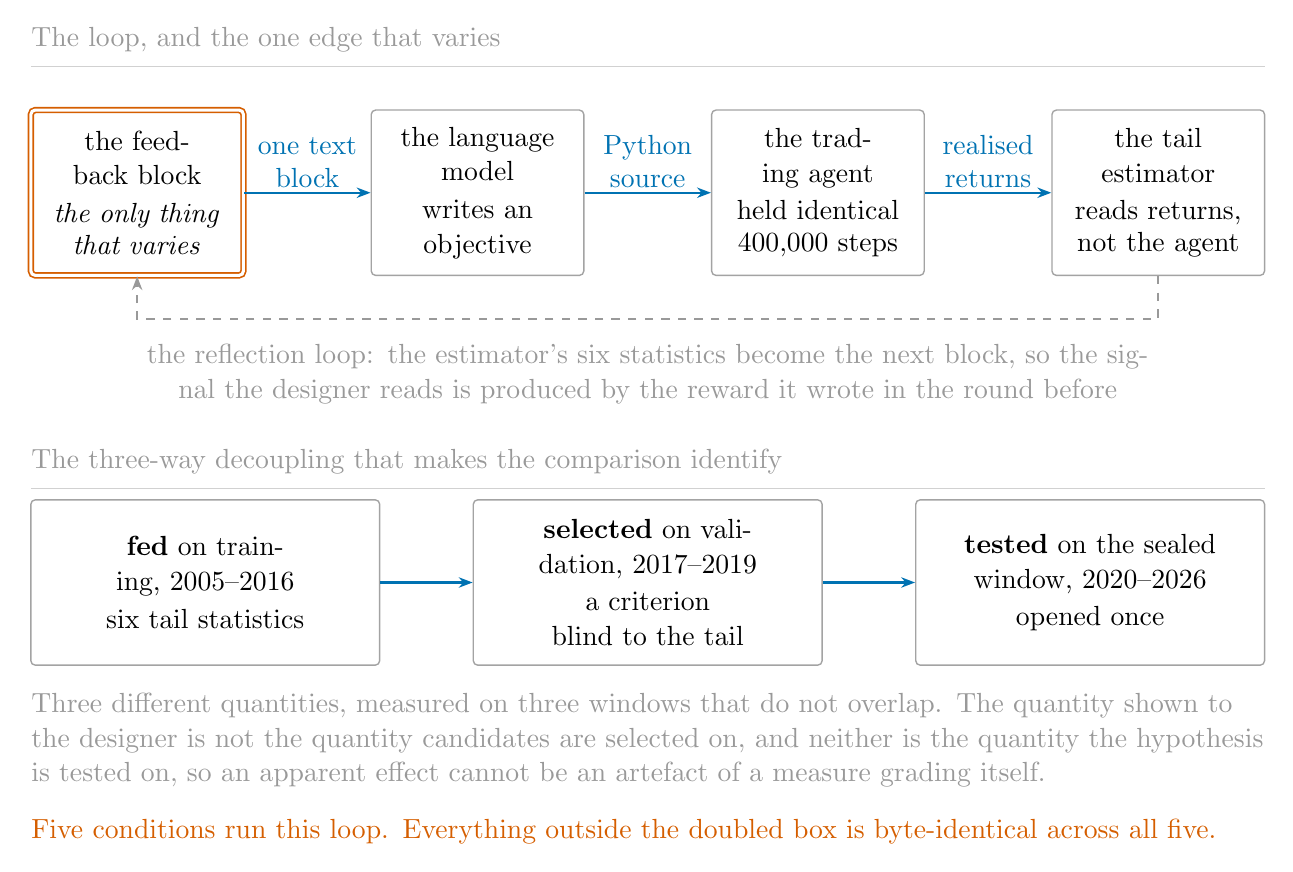
\begin{tikzpicture}[
  >={Stealth[length=5pt]},
  font=\fontsize{10bp}{12.5bp}\selectfont,
  box/.style   ={draw=oiGrey!90, fill=white, rounded corners=1.6pt, align=center,
                 inner sep=3pt, line width=0.5pt},
  vary/.style  ={draw=oiVerm, fill=white, rounded corners=1.6pt, align=center,
                 inner sep=3pt, line width=0.6pt,
                 double, double distance=1.1pt},
  flow/.style  ={->, draw=oiBlue, line width=0.8pt},
  loop/.style  ={->, draw=oiGrey, line width=0.7pt, dashed},
  dim/.style   ={inner sep=1.5pt, text=oiBlue, align=center,
                 font=\fontsize{10bp}{12bp}\selectfont},
  note/.style  ={inner sep=0pt, text=oiGrey, align=center,
                 font=\fontsize{10bp}{12.5bp}\selectfont},
  sect/.style  ={inner sep=0pt, text=oiGrey, font=\fontsize{10bp}{12bp}\selectfont},
]

% ---- the grid, stated once ---------------------------------------------------------
% \W is the printed column: 453.5 pt less the 4 pt standalone border on each side is
% 445.5 pt = 15.71 cm. Row A is four boxes on that width; whatever the boxes do not
% take becomes the channel the arrow dimensions are set in, so the two are never fitted
% independently and can never overlap by arithmetic.
\pgfmathsetmacro{\W}{15.668}
\pgfmathsetmacro{\boxwd}{2.70}                 % row-A box width
\pgfmathsetmacro{\chan}{(\W-4*\boxwd)/3}       % row-A channel = 1.64 cm
\pgfmathsetmacro{\pitch}{\boxwd+\chan}
\pgfmathsetmacro{\xa}{\boxwd/2}
\pgfmathsetmacro{\xb}{\xa+\pitch}
\pgfmathsetmacro{\xc}{\xa+2*\pitch}
\pgfmathsetmacro{\xd}{\xa+3*\pitch}
\pgfmathsetmacro{\boxwdB}{4.43}                % row-B box width
\pgfmathsetmacro{\chanB}{(\W-3*\boxwdB)/2}
\pgfmathsetmacro{\xp}{\boxwdB/2}
\pgfmathsetmacro{\xq}{\xp+\boxwdB+\chanB}
\pgfmathsetmacro{\xr}{\xp+2*(\boxwdB+\chanB)}

% ============================================================ SECTION A
\node[sect, anchor=west] at (0,0.34) {The loop, and the one edge that varies};
\draw[oiGrey!45, line width=0.4pt] (0,0) -- (\W,0);

% Geometry note: the four boxes leave a 1.64 cm channel between edges, and every
% dimension label is set on two lines so it fits inside that channel. The 7 pt proof
% used one-line labels and every one of them collided with a box; at 10 pt the break
% has to fall one word earlier still.
% A COMMON minimum height across the row, not a per-box one: the middle box of section B
% needs a fourth line and the others do not, and boxes centred on one baseline with
% different heights read as a mistake rather than as a difference.
\node[vary, minimum width=\boxwd cm, text width=2.25cm, minimum height=21mm] (blk) at (\xa,-1.60)
  {the feedback block\\[1pt]\textit{the only thing}\\[-1pt]\textit{that varies}};
\node[box, minimum width=\boxwd cm, text width=2.25cm, minimum height=21mm] (llm) at (\xb,-1.60)
  {the language model\\[1pt]writes an objective};
\node[box, minimum width=\boxwd cm, text width=2.25cm, minimum height=21mm] (agt) at (\xc,-1.60)
  {the trading agent\\[1pt]held identical\\[-1pt]400{,}000 steps};
\node[box, minimum width=\boxwd cm, text width=2.25cm, minimum height=21mm] (est) at (\xd,-1.60)
  {the tail estimator\\[1pt]reads returns,\\[-1pt]not the agent};

\draw[flow] (blk) -- node[dim, above]{one text\\block} (llm);
\draw[flow] (llm) -- node[dim, above]{Python\\source} (agt);
\draw[flow] (agt) -- node[dim, above]{realised\\returns} (est);

% The reflection loop is drawn and explained rather than implied. The route runs BELOW
% the row and the note sits below the route, because the first proof ran the note
% straight through the dashed line and the boxes.
\draw[loop] (est.south) -- (\xd,-3.20) -- (\xa,-3.20) -- (blk.south);
\node[note, anchor=north, text width=\W cm] at (\W/2,-3.52)
  {the reflection loop: the estimator's six statistics become the next block, so the signal the
   designer reads is produced by the reward it wrote in the round before};

% ============================================================ SECTION B
\node[sect, anchor=west] at (0,-5.02) {The three-way decoupling that makes the comparison identify};
\draw[oiGrey!45, line width=0.4pt] (0,-5.36) -- (\W,-5.36);

\node[box, minimum width=\boxwdB cm, text width=3.98cm, minimum height=21mm] (tr) at (\xp,-6.55)
  {\textbf{fed} on training, 2005--2016\\[1pt]six tail statistics};
\node[box, minimum width=\boxwdB cm, text width=3.98cm, minimum height=21mm] (va) at (\xq,-6.55)
  {\textbf{selected} on validation, 2017--2019\\[1pt]a criterion blind to the tail};
\node[box, minimum width=\boxwdB cm, text width=3.98cm, minimum height=21mm] (te) at (\xr,-6.55)
  {\textbf{tested} on the sealed window, 2020--2026\\[1pt]opened once};

\draw[flow] (tr) -- (va);
\draw[flow] (va) -- (te);

\node[note, anchor=north west, align=left, text width=\W cm] at (0,-7.95)
  {Three different quantities, measured on three windows that do not overlap. The quantity shown to the
   designer is not the quantity candidates are selected on, and neither is the quantity the hypothesis is
   tested on, so an apparent effect cannot be an artefact of a measure grading itself.};

\node[anchor=north west, align=left, inner sep=0pt, text width=\W cm, text=oiVerm,
      font=\fontsize{10bp}{12.5bp}\selectfont] at (0,-9.55)
  {Five conditions run this loop. Everything outside the doubled box is byte-identical across all five.};

\end{tikzpicture}
\end{document}
